\subsection{Background} %Anette
Since the robot is to be submerged, some kind of water protection was required for the electronics. The solution in Naiad is a watertight chamber for the electronics. Also the motors need to be mounted on something. The previous team had constructed the main hull and with that decided how this chamber as well as the thruster configuration were to look. 

	\subsubsection{Main hull} %Martina
	\noindent At the beginning of this project, the main hull was already milled and all six motors were mounted. There were also compressing spring latches mounted on the hull for the purpose of attaching the lid of the main hull. 

One side of the hull has two differently shaped countersinks which are intended for holding a kill switch and a mission switch. The lid has a window for viewing an LCD display which may show status messages to the user when the robot is operating. The window consists of a clear Polymethylmethacrylate (PMMA) plastic which has an O-ring between itself and the lid to secure a waterproof system. 

There is also an O-ring track around the top edge of the hull to further waterproof the system with a custom-made O-ring. Furthermore, there are two camera housings built into the hull, one facing forward and the other facing downward. These camera housings have, like the window on the lid, plates of transparent PMMA so that the surroundings can be observed by the cameras from inside of the hull.

At the bottom of the hull there are four tapped holes for the purpose of being able to have e.g. an Ethernet cable through the hull for manual control of Naiad or for connecting peripherals from outside of the hull. 

	\subsubsection{Thruster configuration} %Ande
	
To allow Naiad to move underwater in all three directions x, y and z and to control all three orientations, roll pitch and yaw, six thrusters were mounted. This is the minimal number of thrusters to the six degrees of freedom. The configuration of the thrusters was made by the previous group and it was their belief that this configuration to be more agile and responsive than the configuration Vasa had \cite{Vasadoc}. However the thrusters were never tested in the water by the previous group.

	\begin{figure}[!ht]
	\begin{center}
		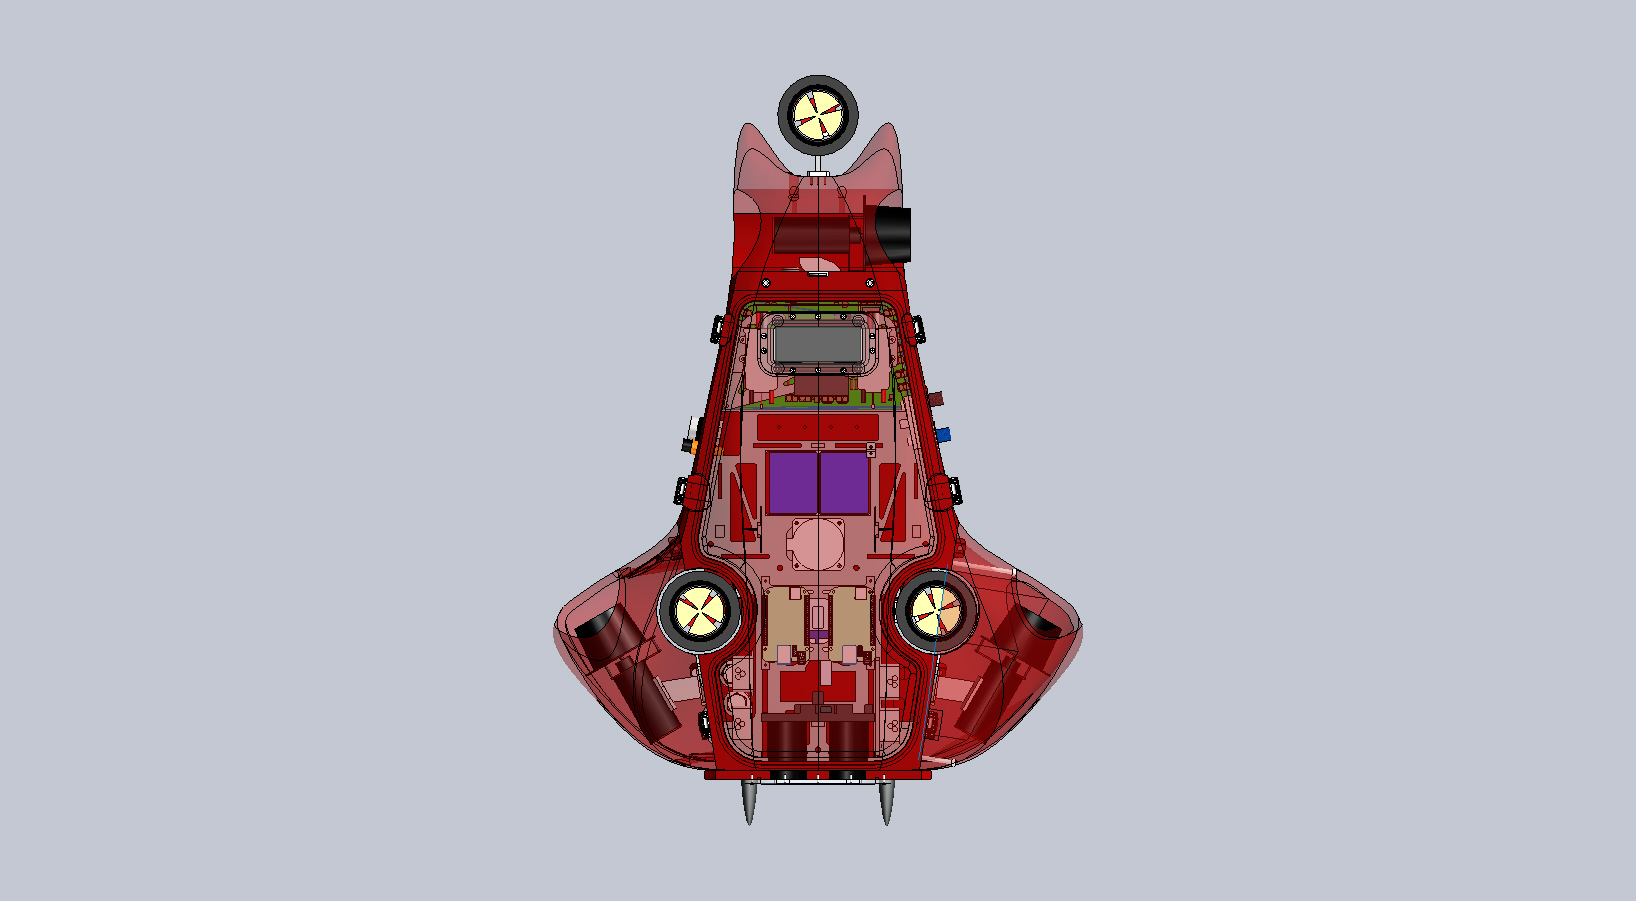
\includegraphics[width=120mm]{./images/mechanics/thcon.png}
		\caption{The six thrusters which allows NAIAD AUV to get the six degrees of freedom.}
		\label{thcon}
	\end{center}
\end{figure}

The previous group, using the Solidwork model, created a matrix of the relative effect of each thruster on each component, this can be seen in fig. \ref{matrix}. The matrix were used to convert the thrusters value from the optimal thruster to the real thruster configuration.

	\begin{figure}[!ht]
	\begin{center}
		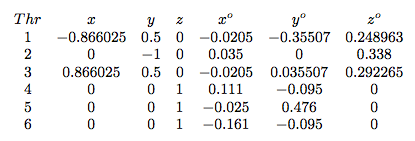
\includegraphics[width=120mm]{./images/mechanics/matrix.png}
		\caption{The configuration Matrix. Figure \ref{matrixindex} below explains the index.}
		\label{matrix}
	\end{center}
\end{figure}

	\begin{figure}[!ht]
	\begin{center}
		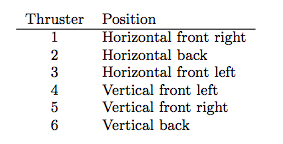
\includegraphics[width=80mm]{./images/mechanics/matrixindex.png}			\caption{Thruster indices}
		\label{matrixindex}
	\end{center}
	\end{figure}

\subsubsection{Toolplate}

The previous group had also designed a prototype of how the design of the tool plate and front tool plate could look. This design however was not finish to be manufactured. The design suggested also where the pneumatic box and the gripper could be placed, see fig. \ref{Toolplate} below. There where also a prototype of how the gripper and the pneumatic box could look like, but neither designs were not ready to be manufactured. Both had to be redesigned.

	\begin{figure}[!ht]
	\begin{center}
		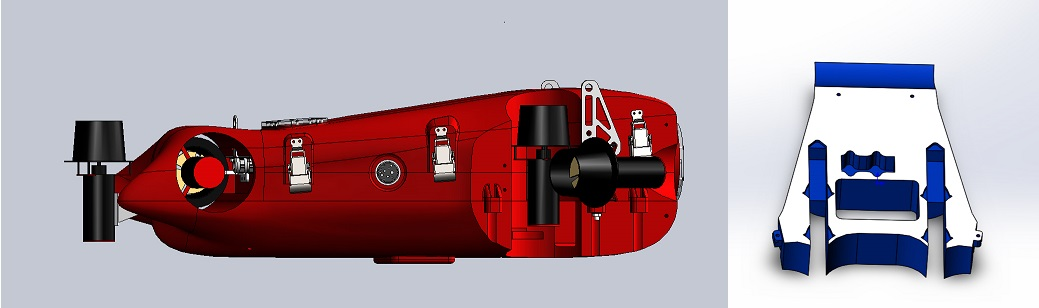
\includegraphics[width=150mm]{./images/mechanics/Naiadassembly.JPG}
		\caption{The old design of tool plate.}
		\label{Toolplate}
	\end{center}
	\end{figure}
	
	
 